\section{Exploring Interleaving Space}
\label{s:design}

In order to test whether threads cause a concurrency bug or not, the
straightforward method is to run the threads iteratively while
\textit{diversifying thread interleaving across iterations} until the
threads \textit{do not expose new interesting thread interleaving}.


In this section, we describe our approach to effectively explore the
search space of thread interleaving.
%
We first describe the key idea of our
approach~(\autoref{ss:overview}). Then, we illustrate our coverage
metric in the concurrency dimension~(\autoref{ss:coverage}), and the
instruction scheduling algorithm to quickly saturate the
coverage~(\autoref{ss:scheduler}).



While this section focuses only on exploring the search space of
thread interleaivng of given threads, \autoref{s:impl} describes the
whole design of \sys for expanding both code coverage and interleaving
coverage.


\subsection{Key Idea}
\label{ss:overview}

\begin{figure}[t]
  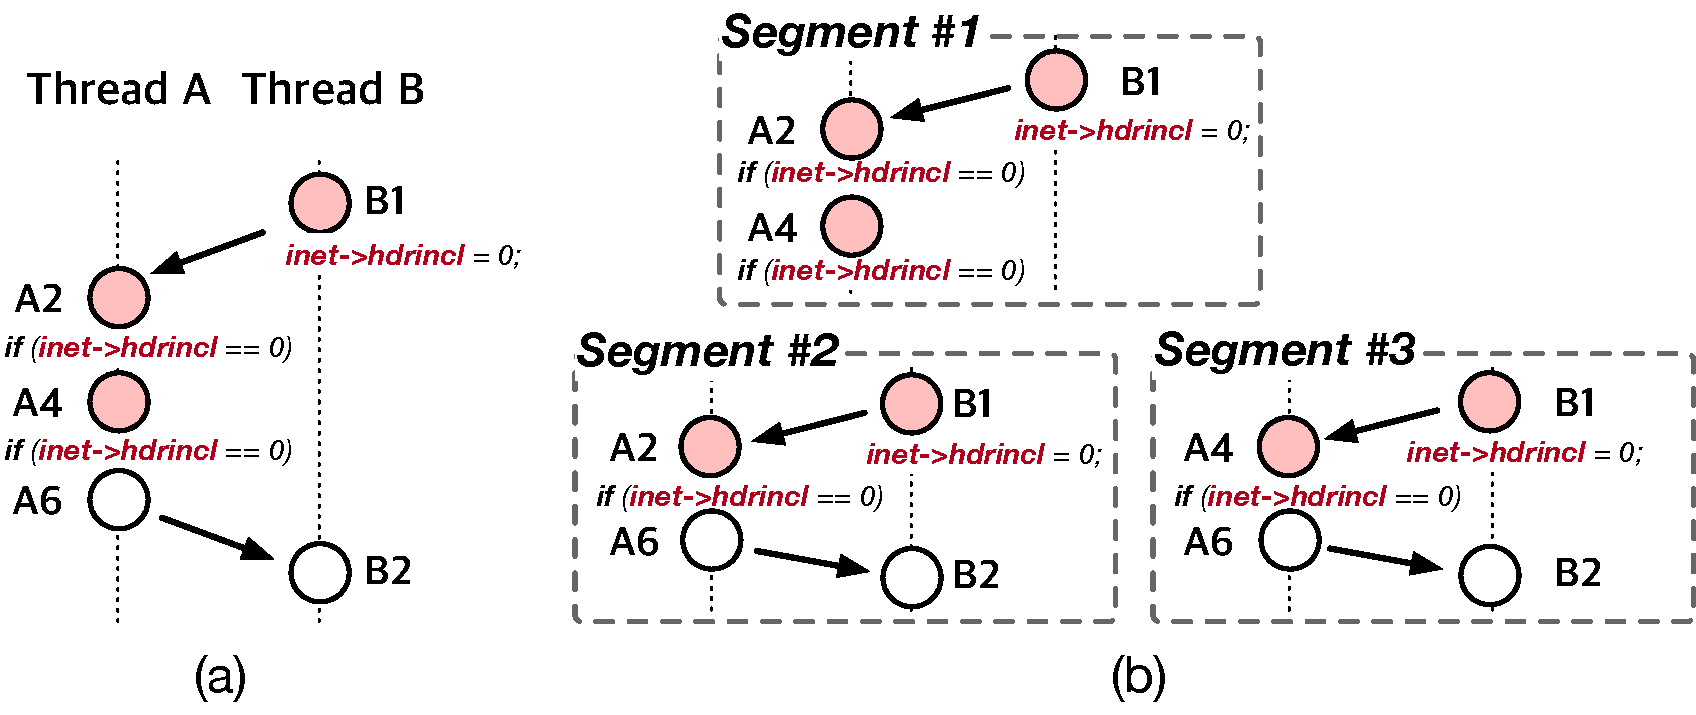
\includegraphics[width=0.9\linewidth]{fig/intuition.pdf}
  \caption{Approach overview to explore the interleaving
    space.}
  \label{fig:keyidea}
\end{figure}
%
The key idea of our approach is to consider an instance of thread
interleaving as \textit{a composition of interleaving segments}, where
each interleaving segment represents the execution order of a small
number of memory accesses.
%
In particular, after executing threads concurrently, we firstly model
an execution of these threads as a totally-ordered instruction
sequence.
%
And then, we group a small number of instructions (\eg, four
instructions) as a segment to track which segments are contained in
the execution and search for other segments in future iterations.


\autoref{fig:keyidea} visualizes our key idea.
%
In this example, let us assume we are testing whether thread
interleaving of the two system calls, \texttt{Syscall A} and
\texttt{Syscall B}, causes a concurrency bug.
%
While executing the two system calls, we track memory access
operations conducted by the two system calls with timestamps, and
construct a totally-ordered instruction sequence as described in
\autoref{fig:keyidea}-(a).

we can decompose the interleaving instance into three interleaving
segments as described in \autoref{fig:keyidea}-(b).


It is worth noting that segments can be overlapped; in this example,
\texttt{Segment \#1} and \texttt{Segment \#2} are overlapped over XXX.





\PP{Benefits}
%
This approach provides two remarkable benefits.
%
\textbf{i)} Tracking interleaving segments is a befitting choice to
determine if any \textit{interesting} thread interleaving remains.
%
According to the extensive survey conducted by Shan Lu
\etal~\cite{learningfrommistakes}, most (\ie, more than 90\%)
concurrency bugs manifest depending on the execution order of a small
number (mostly, four) of memory accesse.
%
In this perspective, whether or not an interleaving instance causes a
concurrency bug depends on whether a problematic segment is contained
in the instance of thread interleaving.
%

\textbf{ii)} interleaving segments contained in an iteration gives
promising hints for diversifying thread interleaving in future
iterations.
%
In other words, with a given interleaving segment, we can rearrange
instructions in the interleaving segment to derive \textit{unobserved}
interleaving segment.



\subsection{Interleaving Segment Coverage}
\label{ss:coverage}




\subsection{Coverage-directed Interleaving Mutation}
\label{ss:scheduler}


%%% Local Variables:
%%% mode: latex
%%% TeX-master: "p"
%%% End:
